%Publication version
% \documentclass[aps,twocolumn,prd,superscriptaddress,showpacs,nofootinbib,fixfloat]{revtex4-1}
%Draft version
\documentclass[aps,prd,superscriptaddress,showpacs,nofootinbib,fixlfloat, 12pt]{revtex4-1}
%\usepackage{doublespace}
\usepackage{graphicx}
\usepackage{dcolumn}
\usepackage{bm}
\usepackage{natbib}

%\topmargin+1cm

\hyphenation{CTBCORE}

% Journals
\newcommand{\aaps}{{Astron.~Astrophys.~Supp.}}
\newcommand{\physrep}{{Physics~Reports}}
\newcommand{\araa}{{Annu.~Rev.~Astron.~Astrophys.}}
\newcommand{\aap}{{Astron.~Astrophys.}}
\newcommand{\apjl}{{Astrophys.~J.~Lett.}}
\newcommand{\apjs}{{Astrophys.~J.~Supp.}}
\newcommand{\aj}{{Astron.~J.}}
\newcommand{\mnras}{{Mon.~Not.~R.~Astron.~Soc.}}


% Making life easier
\newcommand{\be}{\begin{equation}}
\newcommand{\ee}{\end{equation}}
\newcommand{\bea}{\begin{eqnarray}}
\newcommand{\eea}{\end{eqnarray}}
\newcommand{\backten}{\!\!\!\!\!\!\!\!\!\!}


% useful symbols
\newcommand{\nhat}{\hat{\bf n}}
\newcommand{\kvec}{{\bf k}}
\newcommand{\edm}{\epsilon_{dm}}
\newcommand{\edmnow}{\epsilon_{dm,0}}
\newcommand{\sv}{\langle\sigma_Av\rangle}
\newcommand{\khat}{\hat{\bf k}}

% Fermi is usually italicized - use \Fermi\ for space after word
\newcommand{\Fermi}{{\slshape Fermi}}

% math functions, units
\newcommand{\Mpc}{{\rm ~Mpc}}
\newcommand{\sech}{{\rm ~sech~}}
\newcommand{\Tr}{{\rm ~Tr~}}
\newcommand{\threej}[6]{{\left( \begin{array}{ccc} #1 & #2 & #3 \\ #4 & 
   #5 & #6 \end{array} \right)}}

% Doug's units
\newcommand{\s}{{\rm ~s}}
\newcommand{\kms}{{\rm ~km/s}}
\newcommand{\g}{{\rm ~g}}
\newcommand{\cm}{{\rm ~cm}}
\newcommand{\ph}{{\rm ~ph}}
\newcommand{\sr}{{\rm ~sr}}
\newcommand{\km}{{\rm ~km}}
\newcommand{\mm}{{\rm ~mm}}
\newcommand{\mJy}{{\rm ~mJy}}
\newcommand{\Jy}{{\rm ~Jy}}
\newcommand{\MJy}{{\rm ~MJy}}
\newcommand{\MJypSr}{{\rm ~MJy~sr^{-1}}}
\newcommand{\JypSr}{{\rm ~Jy~sr^{-1}}}
\newcommand{\Hz}{{\rm ~Hz}}
\newcommand{\kHz}{{\rm ~kHz}}
\newcommand{\MHz}{{\rm ~MHz}}
\newcommand{\GHz}{{\rm ~GHz}}
\newcommand{\K}{{\rm ~K}}
\newcommand{\mK}{\rm ~mK}
\newcommand{\microK}{\mu{\rm K}}
\newcommand{\eV}{{\rm ~eV}}
\newcommand{\eVs}{{\rm ~eV/s}}
\newcommand{\keV}{{\rm ~keV}}
\newcommand{\MeV}{{\rm ~MeV}}
\newcommand{\GeV}{{\rm ~GeV}}
\newcommand{\TeV}{{\rm ~TeV}}
\newcommand{\pc}{{\rm ~pc}}
\newcommand{\kpc}{{\rm ~kpc}}
%\newcommand{\Mpc}{{\rm ~Mpc}}
\newcommand{\erg}{{\rm ~erg}}
\newcommand{\degree}{^{\rm o}}
\newcommand{\sigmav}{\langle\sigma_Av\rangle}
\newcommand{\zrock}{$Z_{\rm rock}$}
\newcommand\reftbl[1]{Table \ref{tbl:#1}}
\def\la{\vcenter{\hbox{$<$}\offinterlineskip\hbox{$\sim$}}}
\def\ga{\vcenter{\hbox{$>$}\offinterlineskip\hbox{$\sim$}}}
\newcommand\Refsec[1]{Section \ref{sec:#1}}

% Necessary for appendices

%% \newcommand\dpf[1]{{\bf (DPF: #1)}}
%% \newcommand\dpf[1]{{\bf (MS: #1)}}
%% \newcommand\dpf[1]{{\bf (CW: #1)}}

\begin{document}


\title{Fermi White Paper}

\author{Douglas P. Finkbeiner}
%\email{dfinkbeiner@cfa.harvard.edu}
\affiliation{Institute for Theory and Computation,
  Harvard-Smithsonian Center for Astrophysics, 
  60 Garden Street, MS-51, Cambridge, MA 02138, USA} 
\affiliation{Center for the Fundamental Laws of Nature,
  Physics Department, 
  Harvard University, 
  Cambridge, MA 02138 USA}

\author{Meng Su}
\affiliation{Institute for Theory and Computation,
  Harvard-Smithsonian Center for Astrophysics, 
  60 Garden Street, MS-51, Cambridge, MA 02138, USA} 
\affiliation{Department of Physics, and Kavli Institute for Astrophysics and Space Research, Massachusetts Institute of Technology, Cambridge, MA 02139, USA}
\affiliation{Einstein Fellow}

\author{Christoph Weniger}
\affiliation{Amsterdam}

\author{Nestor Mirabel}
\affiliation{affil}

%% Claims of a line are important and demand a careful search for
%% systematics.  Limb photons provide a reference spectrum and look a bit
%% fishy.  Need more data.
\begin{abstract} Does a white paper have an abstract?
\end{abstract}

\pacs{95.35.+d}

\maketitle


%%%%%%%%%%%%%%%%%%%%%% SECTION I %%%%%%%%%%%%%%%%%%%%%%%%%%%%%%%

\section{Introduction}


The search for non-gravitational signatures from WIMP
(weakly interacting massive particle) dark matter has 
generally been approached from three different directions: missing
energy searches at colliders, direct searches for the
recoil of nuclei from underground detectors, and indirect
methods including searching for dark matter signals from cosmic
rays (CR) and multiwavelength astronomical
observations~\citep{Jungman:1995df, Bergstrom:2000, Bertone:2005, Hooper:2007Review,
2012arXiv1205.4882B, Cirelli:2012tf}.

For indirect detection, distinguishing the dark matter
signal from conventional astrophysical backgrounds is
challenging
(for a recent review on indirect searches with gamma rays
see~\cite{Bringmann:2012ez}).
Among various possible signatures, gamma-ray
line emission is a long-sought ``smoking
gun'' for dark matter annihilation~\cite{Bergstrom:1988fp}, as no plausible
astrophysical background can produce such a line
signature.\footnote{A narrow feature is
possible in theory~\citep[see][]{2012arXiv1207.0458A}.}  Gamma-ray line(s)
could be produced by dark matter decays or annihilations
into two photons, or two-body final states involving one
photon plus a Higgs boson, Z boson, or other neutral non-SM
particle.  In most models, the branching ratio
to lines is loop suppressed relative to the continuum
emission, and one would have expected to see the continuum
first in e.g. MSSM models~\citep[e.g.][]{Bergstrom:1997}.
Although this theoretical prejudice led most previous
studies to focus on continuum searches, there are models
being proposed that allow high line to continuum
ratios~\citep[e.g.][]{Bergstrom:1998, Bergstrom:2000,
Bertone:2009, Jackson:2010, Cline:2012, Weiner:2012}.
However, previous searches in EGRET~\cite{Pullen:2006sy} and \Fermi-LAT
data~\cite{Abdo:2010nc, Vertongen:2011mu, Ackermann:2012qk}
did not find any
indications for a gamma-ray line signal and presented only upper limits on the
line flux.

The first claims for a spectral feature around 130 GeV were made by Bringmann
\textit{et al.}~\citep{Bringmann:2012} and Weniger~\citep{Weniger:2012}. While
Ref.~\citep{Bringmann:2012} mostly concentrated on an interpretation in the context of
virtual internal Bremsstrahlung signals from annihilations,
Ref.~\citep{Weniger:2012} focused on gamma-ray lines and a thorough discussion
of possible instrumental effects.  Both works performed a spectral fit to
photon events in regions of interest in
the inner Galaxy designed to maximize S/N. The significance of the line structure
at 130 GeV was found to be 4.6$\sigma$, or 3.2$\sigma$ after the trials factor
correction~\citep{Weniger:2012}.
This claim was quickly followed up and disputed by a number of
groups~\cite{tempel:2012ey, Boyarsky:2012ca}.

Subsequent work by Su \& Finkbeiner approached the problem
with template fitting, which takes into account the spatial
distribution of events along with spectral information,
assuming various profiles (Einasto, NFW, Gaussian) for the
DM distribution~\citep{linepaper}.  If the template is
correct, this allows extraction of the DM signal with higher
S/N.  This work found 6.6$\sigma$ (5.1$\sigma$ after the
trials factor correction) for an Einasto profile centered
$1.5\degree$ west of the Galactic center, and also suggested
that there may be two lines, at about 111 and 129 GeV.  The
lower energy line is tantalizing because it matches the
expected energy of a $Z\gamma$ line if the higher energy is
the $\gamma\gamma$ line.  These findings have inspired a
number of models and further analysis of the \Fermi\
data~\citep{Dudas:2012, Choi:2012, Kyae:2012, Lee:2012,
Rajaraman:2012, Acharya:2012, Garny:2012, Buckley:2012,
Chu:2012, Kang:2012, Buchmuller:2012, Bergstrom:2012b,
Heo:2012, Park:2012, Tulin:2012, Cline:2012, Weiner:2012,
WeinerYavin:2012b, FanReece:2012, Huang:2012, Whiteson:2012,
Buchmuller:2012, Cholis:2012}.

Recent evidence for lines at 111 GeV and 129 GeV with a
local significance of $3.3\sigma$ from \Fermi\ unassociated
point sources suggests an annihilation signal is
present~\cite{doubleline}\citep[but
see][]{HooperLinden:2012b}, as does the claim of line
emission from galaxy clusters at 130
GeV~\cite{Hektor:2012kc}.  Neither of these would stand on
their own, but they provide support for the hypothesis that
the Galactic center line signal is produced by dark matter
annihilation.

The high statistical significance of the line feature
motivates a search for systematic errors in the LAT data
that could mimic a line in the Galactic center.
Confirmation by Imaging Air Cherenkov Telescopes like
HESS-II might be possible as early as next
year~\cite{Bergstrom:2012}, but in the meantime a thorough
study of LAT systematics is urgently needed.  We do not have
access to the details of the reconstruction of each photon
event, which would allow us to study how it developed in the
tracker and calorimeter.  However, we do have information
about each event from the public event lists and spacecraft
parameter files.  We can use this information to search for
any line-producing artifacts in the detector frame, and
investigate if they could map onto the Galactic center.

The Earth's atmosphere provides a convenient source of
photons for systematics tests.  The continual cosmic-ray
cascades in the Earth's atmosphere produce gamma rays with
$dN/dE \sim E^{-2.8}$~\citep{FermiLimb}.  Because these
so-called `Earth limb photons' result from atmospheric
cascades, they are produced by interactions in a highly
boosted frame, and cannot contain line emission.
\medskip


\begin{figure}[h]
  \begin{center}
    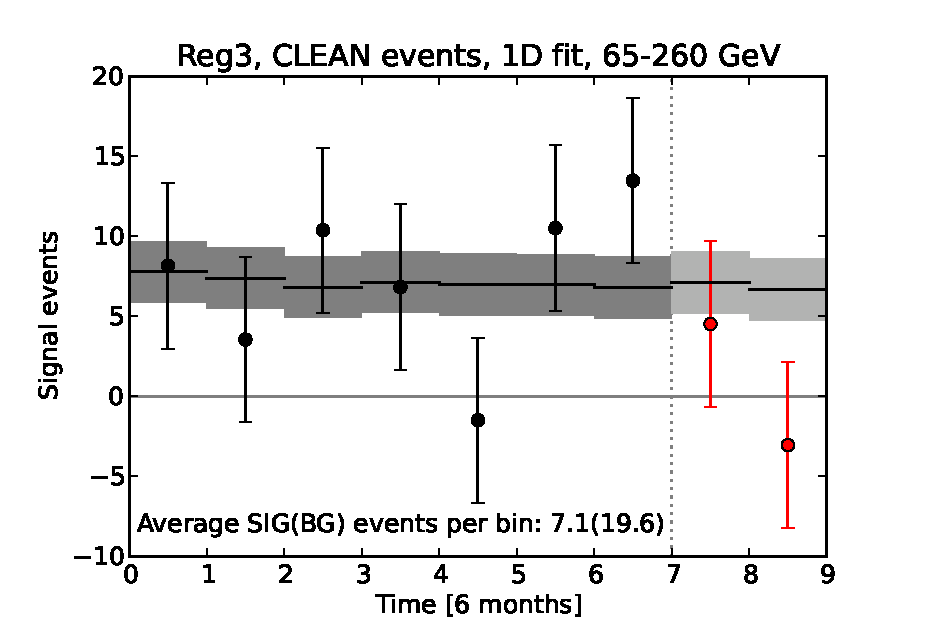
\includegraphics[width=0.60\linewidth]{plots/semester_fluxes.eps}
    \vspace{-0.5cm}
  \end{center}
  \caption{Number of signal events in 6-month bins starting from 4
    August 2008, obtained by an unbinned likelihood fit to the data in
    Region~3 of Ref.~\cite{Weniger:2012}. The gray band shows the expected
    signal rate with $\pm1\sigma$ uncertainty as extracted from data taken until
    4 February 2012; the mild variations stem from variations of the
    exposure. In red we show data taken since 4 February 2012
    together with the projected event rate.}
  \label{fig:semester_fluxes}
\end{figure}


\begin{figure}[h]
  \begin{center}
    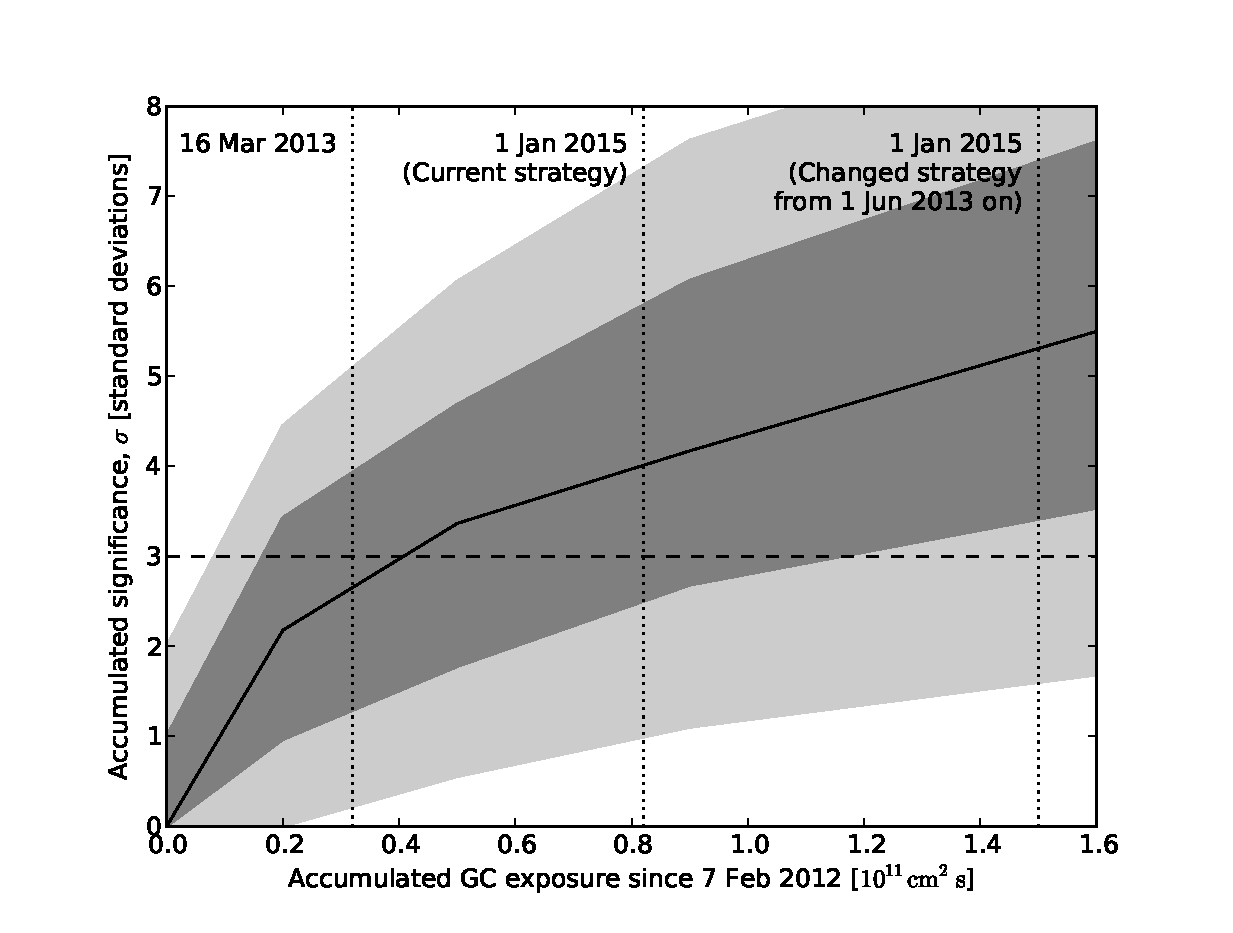
\includegraphics[width=0.6\linewidth]{plots/projection.eps}
    \vspace{-0.5cm}
  \end{center}
  \caption{
    Expected evolution of signal significance in Region~3 from
    Ref.~\cite{Weniger:2012}, starting on 4
    February 2012, as function of
    accumulated exposure.  The shaded bands show $68\%$ and $95\%$ CL
    uncertainties as derived from a Monte Carlo simulation.  The assumed
    signal rate is $1.2\pm 0.3$ events per month, the effective background is
    $3.3$ events per month (the values measured prior to 4 February 2012).
    The first and second vertical dotted lines indicate how much exposure is
    expected to be accumulated until end of 2014 if the observation strategy remains
    unchanged, and respectively when the observation strategy proposed in this
    white paper is adopted starting from June 2013.}
  \label{fig:projection}
\end{figure}

\begin{figure}[h]
  \begin{center}
    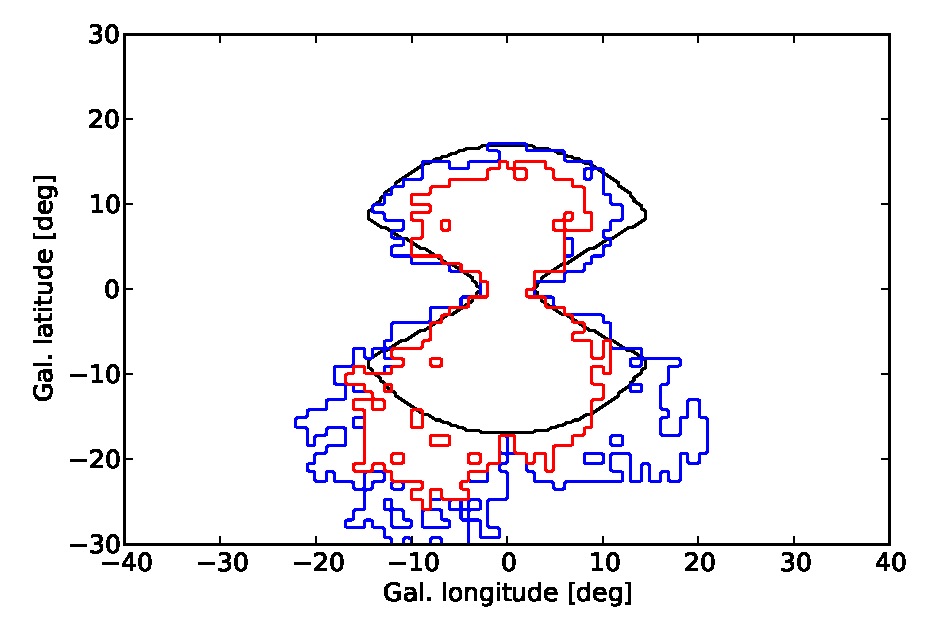
\includegraphics[width=0.6\linewidth]{plots/regions.eps}
    \vspace{-0.5cm}
  \end{center}
  \caption{Region 3 (blue) and Region 4 (red) used in
    Ref.~\cite{Weniger:2012}, together with the simpler hourglass region
    proposed for future studies.}
  \label{fig:projection}
\end{figure}


\section{Current situation and projection}
\subsection{The Galactic center feature}
In Fig.~1 we show the temporal distribution of tentative signal events 
during the last 4.5 years of data taking.
Starting at 4 August 2008, each bin corresponds to a time interval
of six month. The first 7 bins show to data taken prior to the
publication of Ref.~\cite{Bringmann:2012}, the red data points are data taken
since then.  Fits to the data are performed in Region 3 from
Ref.~\cite{Weniger:2012}, using an energy range from 65 to 260 GeV, fixing the
line position at $E_\gamma=129.8\rm\,GeV$, and using P7CLEAN events only. The
details of the fit are identical what was done in Ref.~\cite{Weniger:2012},
but we checked that similar results are obtained using Region 4,
P7SOURCE events, or a 2D fit that takes into account incidence angle as well
as energy information in the modeling of the line. 

The number of signal events $N_s$ in each bin follows directly from a fit to
the data. The effective number of background events is estimated by $N_b =
N_s^2/s^2$, where $s$ is the significance of the signal in units of
standard deviations. The error-bars are
given by $\Delta N_s = \sqrt{N_s+N_b}\simeq5.2$. For comparison, the gray
bands show the number of signal events expected from a fit to 3.5 years of
data: on average $N_s=7.1\pm 1.8$ events per bin, with
mild variations being related to the exposure. The last two
bins are compatible with both the signal- and the null-hypothesis at the two
sigma level (see also Ref.~\cite{Weniger:2013dya}). \medskip

In Fig.~2 we shows 68\% and 95\% CL bands for the projected evolution of the signal significance as
function of exposure accumulated after 4 February 2012. 
To generate the plot, we simulate events from a
power-law plus line model and derive the signal significance for each
realization as described above. The background and signal correspond to the
best-fit values obtained in Region 3 with data until 4 February 2012.  For
different realizations we allow the signal normalization to vary following a
normal distribution that is matched to the $\pm1\sigma$
flux uncertainties from the 3.5 year results. We checked that similar results
are obtained for Region 4, or in the hourglass region discussed below.

The first vertical dashed line indicates the exposure that will be acquired
until end of next year. It is likely that a true signal would be confirmed
with $>3\sigma$ significance, although this is not guaranteed due to the
$95\%$ CL error bands that range down to significances of only $1\sigma$. What
is more, it will be difficult to robustly rule out the signal hypothesis at
the $3\sigma$ level unless the accumulated significance will be close to zero.
As we will discuss in the next section, a change in the observation strategy
will allow a much quicker confirmation/rejection of the signal hypothesis.

\medskip
For future analysis of the 130 GeV feature in the LAT data, instead of using the difficult to reproduce regions from
Ref.~\cite{Weniger:2012}, we propose to use the region shown in black in
Fig.~3. This region is defined in $(\ell, b)$ space as the intersection of
$\ell^2+b^2\leq r^2$ and $\ell^2\leq (b\tan\varphi)^2 + d^2$, with $(r,
d, \varphi) = (20^\circ, 3^\circ, 60^\circ)$, and has similar signal-to-noise
properties as Region 3 or 4. 
% In particular, Fig.~2 is also valid for that region.

\subsection{The Earth limb feature}
The most direct indication for an instrumental cause of the Galactic center
feature is an excess of 130 GeV photons in low incidence angle events from
the Earth limb~\cite{linepaper, finkbeiner_systematics, Hektor:2012ev,
bloom_charles_fermi_lat_line}. Although it is challenging to understand how
such a feature could possibly be mapped onto the Galactic center while being
absent in other test regions, this feature raised serious concerns about the
energy reconstruction of the LAT around 130 GeV. More data is required to
determin whether the Earth limb feature is indeed a true systematic effect or
merely a statistical fluke in light of a large number of hidden trials.

We define here the Earth limb excess by selecting P7CLEAN events until 5 Sep 2012 at zenith angles $Z>100^\circ$,
incidence angles $\theta<60^\circ$, and excluding events within $20^\circ$ of
the Galactic center. In this data set, the line feature at 130~GeV has a
significance of $2.7\sigma$ when
adopting an energy range from 65--260~GeV in the fit (for details of the assumed line shape etc
see Ref.~\cite{finkbeiner_systematics}).\footnote{If we take into account data
  until 16 Apr 2013, the
significance of the Earth limb feature is marginally larger, namely
$3.0\sigma$.} Data accumulated after 5 Sep 2012 can
now be used to test whether this excess is a fluke or not. Using the above
cuts, we find that the rate of events above 100 GeV that were accumulated between the
start of the mission and 5 Sep 2012 is 9.5 ph/month (in total 474), whereas it
was 36.7 ph/month between 5 Sep 2012 and 16 Apr 2013. Reason for this increase
in the rate are the start of weekly dedicated limb observations as well as two extended
target of opportunity observations in that time period. If the accumulation of
low incidence angle Earth limb data continues at this pace, 2.3 years of fresh
data are enough to regenerate the putative signature with $4.0\sigma$
significance on average, or to rule it out with high significance if it is a
fluke. This amount of data would be available end of 2014.

\section{A New Observation Strategy}
Since start of the mission, Fermi has spend over 95\% of the time in
\emph{standard survey mode}.
% With a field of view of $\sim2.5$~sr, the LAT can survey the entire sky in
% two orbits. 
In this mode, the LAT points north of zenith towards the orbital pole by an
angle \zrock\ on one orbit, and south of zenith by the same angle on the next
orbit; the LAT pointing is confined to the plane perpendicular to its orbital
velocity. 
% The slews are performed with a repeating pattern of 17 waypoints defining
% \zrock\ as a function of time.  \zrock\ was $35\degree$ at the start of the
% nominal mission on August 4, 2008 until May 7th, 2009, and was changed to
% $50\degree$ on September 3rd, 2009 for better thermal management of the
% downward-facing battery radiator.  
This observation profile, combined with the precession of the orbit every
$\sim53.4$ days, allows the LAT to observe the whole sky with approximately
uniform coverage. The standard survey mode is only occasionally interrupted
for pointed observations of targets of opportunity (ToOs). During such times
the LAT may point at larger zenith angle than usual, even at the horizon.  In
addition, survey mode is occasionally interrupted by Autonomous Repoints of
the observatory for triggered gamma-ray burst follow-up observations, and for
calibration.
% Furthermore, \Fermi's survey observations are halted during passages through
% the South Atlantic Anomaly, resulting in an exposure differential between
% north and south of $\sim15$\%. 

However, Fermi is capable of very flexible survey mode patterns. These can
e.g.~alter between survey and pointed observations even within one orbit,
which allows to efficiently increase coverage of certain parts of the sky if
required. We will discuss here in how far this fact can be beneficial for a
study of the 130 GeV feature at the Galactic center. We will
follow here the mixed mode ``option3v3'' proposed by the Fermi
mission.\footnote{See
\url{http://fermi.gsfc.nasa.gov/ssc/proposals/alt_obs/obs_modes.html}.}

We are interested in increasing the exposure of the Galactic center. The basic
strategy would be to switch to pointed observation of the Galactic center as
soon as it gets above horizon, and to follow the standard survey mode
otherwise. More precisely, \Fermi\ would slew from survey mode to the target
once the target is $10^\circ$ from Earth occultation, and slews back to survey
mode position once the target is reentering $10^\circ$ from Earth occultation.
The minimal distance to the Earth horizon (the Earth Avoidance Angle, EAA) is
set to $30^\circ$, to avoid the loss of too much exposure during the
transition periods. 

To reduce potential systematics, it is advisable to avoid point directly at
the target. Instead, it is useful to observe it with a broad distribution of
non-zero incidence angles. In the \emph{mixed observation mode} that we
discuss here, the target is fixed to RA=266.4$^\circ$ and oscillates within
the range Dec=$\pm25.6^\circ$ during one precession period such that the
target lies on the orbital equator. Besides reducing potential systematics,
the variation of the target position yields an improved sky uniformity on
short time scales. 

\subsection{Impact on line searches at the GC}

\begin{figure}[t]
  \begin{center}
    \includegraphics[width=0.49\linewidth]{plots/survey_lineEval.eps}
    \includegraphics[width=0.49\linewidth]{plots/option3v3_lineEval.eps}
    \vspace{-0.5cm}
  \end{center}
  \caption{Evaluation of standard survey mode (\emph{left panels}) and mixed observation
    strategy (\emph{right panels}). Sky maps are in galactic coordinates ($\ell$ increases
    to the left) and averaged over a orbital precession period of 55 days.
    \emph{Top
      panels:} Exposure maps.
    \emph{Central panels:}
    Effective energy resolution.
  \emph{Bottom panels:} Figure of merit for gamma-ray line searches. In all
  panels the overlaid lines show the main axes of the equatorial coordinate
  system; sky maps are symmetric around the Earth equator.}
  \label{fig:mollweide}
\end{figure}

\begin{figure}[t]
  \begin{center}
    \includegraphics[width=0.49\linewidth]{plots/option1v2_lineEval.eps}
    \includegraphics[width=0.49\linewidth]{plots/option2v2_lineEval.eps}
    \vspace{-0.5cm}
  \end{center}
  \caption{Same as Fig.~\ref{fig:mollweide}, but for 'option1v2' and
  option2v2'.}
  \label{fig:mollweide2}
\end{figure}

The upper panels of Fig.~\ref{fig:mollweide} show exposure maps after 55 days
of survey and mixed observation mode in galactic coordinates. As discussed
above, in mixed
observation mode, the point of highest exposure is at (RA,
Dec)$\simeq(266.4^\circ$, $0^\circ)$. At the GC, the exposure
increases by a factor of 2.23 with respect to normal survey mode.

In mixed observation mode, regions close to the GC are predominantly observed
under low incidence angles in the range $\theta=4^\circ$--$54^\circ$ (see
Fig.~\ref{fig:thetaDist}). This has impact on the effective energy resolution
in that direction, which is shown in the central panel of
Fig.~\ref{fig:mollweide}. In direction of the GC the energy resolution is in
fact slightly worsen w.r.t.~standard survey mode: namely $\Delta E/E=9.59\%$
instead of $\Delta E/E=8.75\%$. However, this has only a small effect on line
searches.

As \emph{figure-of-merit} for line searches we define the dimensionless
quantity $Q\equiv a\sqrt{\mathcal{E}/\Delta E}$, which is proportional to the
average expected line significance in units of Gaussian sigma. Here, $a$ is an
arbitrary normalization that we set such that the spatial mean in survey mode
is $\bar Q=1$. In the bottom panel of Fig.~\ref{fig:mollweide} we show sky
maps for $Q$ in mixed and survey mode. At the Galactic center, $Q$ increases
by a factor $1.43$ when switching from survey to mixed mode. Hence, for
gamma-ray lines at the GC, the growth rate of the signal significance is
increased by $40\%$ when switching from survey to mixed observation mode.

\subsection{Impact on other science}

\begin{figure}[t]
  \begin{center}
    % \includegraphics[width=0.49\linewidth, angle=-90]{plots/option1_survey_hist.ps}
    \includegraphics[width=0.49\linewidth, angle=-90]{plots/option2_option3_hist.ps}
    \vspace{-0.5cm}
  \end{center}
  \caption{Histogram on sky pixels of fractional exposure normalized to
  standard survey strategy. Left panel compares the modified strategy option 1
  to the standard survey strategy, and the right panel shows the modified
  strategy option 1 relative to option 3. }
  \label{fig:expHisto}
\end{figure}

In Fig.~\ref{fig:expHisto}, we show as histogram the distribution of exposure
in different pixels of the sky (using a Healpix projection with $N=128$). In
case of standard survey mode, the exposure distribution spans a factor of two,
whereas is spans a factor $12$ in the mixed observation mode. 
% However, only in a small fraction of the sky, about XXX\%, the coverage
% drops by as much as a factor of $0.3$--$0.5$, and never below $0.3$.

For the observation of transient phenomena, it is vital that all parts of the
sky are sufficiently covered at least each day. In Fig.~\ref{fig:coverage} we
show for each individual day of the precession period which fraction of the
sky is covered by what fraction of the mean exposure. As can be seen from the
plot, in less than $\sim5\%$ of the sky the daily coverage drops below $20\%$
of the mean, whereas in $>80\%$ the daily coverage remains above $50\%$ of the
mean.

\begin{figure}[t]
  \begin{center}
    \includegraphics[width=0.38\linewidth, angle=-90]{plots/exposure_pixel_hist_perday_option1.ps}
    \includegraphics[width=0.38\linewidth, angle=-90]{plots/exposure_pixel_hist_perday_option2.ps}
    \includegraphics[width=0.38\linewidth, angle=-90]{plots/exposure_pixel_hist_perday.ps}
    \includegraphics[width=0.38\linewidth, angle=-90]{plots/exposure_pixel_hist_perday_survey.ps}
    \vspace{-0.5cm}
  \end{center}
  \caption{Daily sky coverage with different range of exposure
  time normalized to the mean value of the exposure map of each day (in total
  55 days to complete on orbit precession period).} 
  \label{fig:coverage}
\end{figure}

\begin{figure}[t]
  \begin{center}
    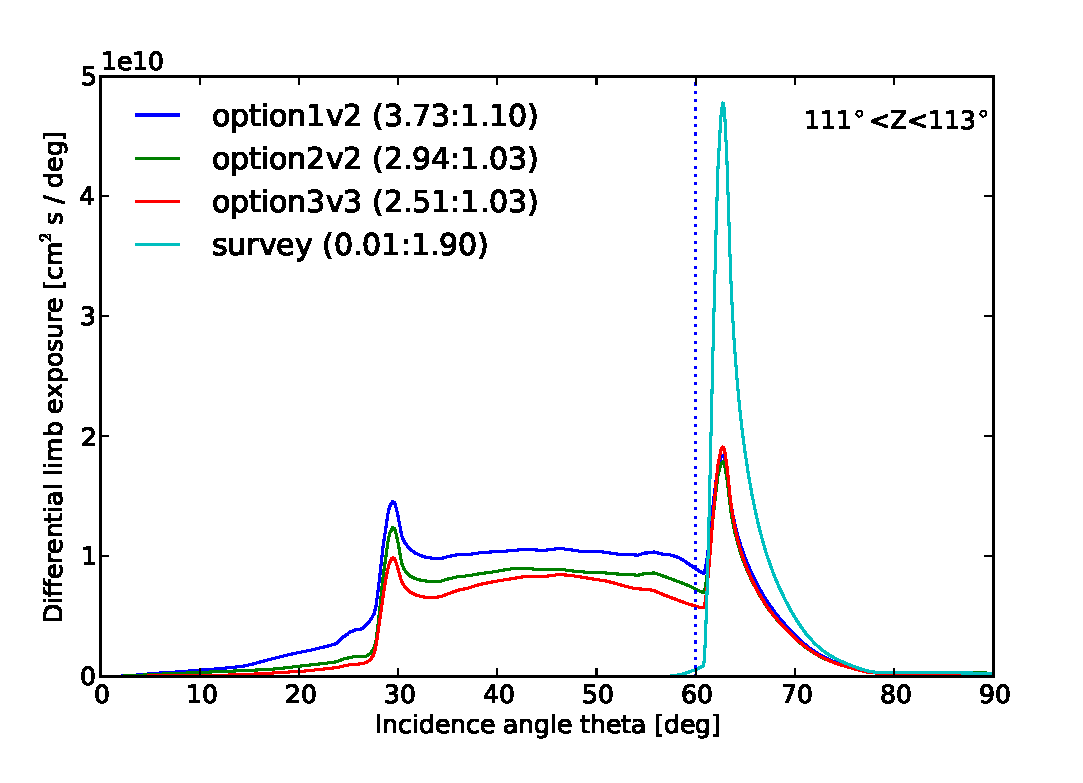
\includegraphics[width=0.6\linewidth]{plots/limb_exposure.eps}
    \vspace{-0.5cm}
  \end{center}
  \caption{Differential exposure of Earth limb region (zenith angles
    $111^\circ<Z<113^\circ$) as function of incidence angle $\theta$. In
    standard survey mode, incidence angles below $\theta<60^\circ$ are not
    exposed to the Earth limb. However, in mixed observation modes, a
    large number of Earth limb events would be collected down to incidence
    angles $\theta\simeq30^\circ$. In brackets we show the exposure below and
  above $\theta=60^\circ$ in units of $10^{11}\rm\,cm^2\,s$.}
  \label{fig:limb_exposure}
\end{figure}

\dots theta distribution at GC (optional) \dots

\begin{figure}[t]
  \begin{center}
    \includegraphics[width=0.49\linewidth, angle=-90]{plots/theta.ps}
    % \includegraphics[width=0.37\linewidth, angle=-90]{plots/exposure_exp_hist_perday.ps}
    \vspace{-0.5cm}
  \end{center}
  \caption{The distribution of Galactic center theta angle. Each entry in the histogram corresponds to a 30 seconds interval. Note that this includes time in the SAA.} %Right panel: in stead the sky
  %coverage, we plot the fractional exposure time relative to the mean value of
  %the exposure map of each day.}
  \label{fig:coverage}
\end{figure}

\section{Discussion and Conclusion}
\label{sec:Conclusion}

In this white paper we have argued for a change in the Fermi strategy on the
following basis.

\begin{itemize}

\item{\bf It is important: discovery of a dark matter annihilation line in the
    Galactic center would be Fermi's greatest accomplishment.}  The nature of
  dark matter is one of the greatest mysteries in physics and astrophysics,
  and the discovery of a line would be a major step forward for both fields.
  Exploring the nature of dark matter is one of the major goals of the Fermi
  project, and a discovery would define Fermi's legacy.

\item{\bf Fermi can do it: a modified survey strategy can obtain a decisive
    measurement, while the status quo cannot.}  I think that 2 years of
  altered survey mode are enough to get a definitive answer.  Calculations we
  have done with Weniger this week show that we need more exposure than I
  thought to get a definitive answer.  If we go with standard survey mode
  until 2016, there is a decent chance that we leave this question unresolved.
  We cannot permit that to happen.

\item{\bf A change is not bad for other science.}  There will be winners and
  losers in any change, but more time on the inner Galaxy is good for lots of
  projects (better time coverage for pulsars and transients, etc.) and it is
  not like we will never observe the rest of the sky.

\item{\bf It looks good for future funding.}  Enough said. 

\end{itemize}

Daniel Eisenstein was both eloquent and forceful about this last point
when we discussed it with him yesterday for an hour.  I'm not sure he
meant to be quoted, but the gist was that there are two possible
scenarios for the situation walking into the senior review:

1.  The LAT saw hints of something that could be its most important
discovery.  The project responded by a call for white papers, decided
to change strategy, and is now N months into a modified survey mode
with a promise of an answer at 99\% confidence by X date.
OR
2.  The LAT saw hints of something that could be its most important
discovery.  The project responded by a call for white papers, and then
did ... nothing.

He was pretty sure option 1 is better for continued funding.  He would
know, since he has done a lot of senior reviewing himself.  I know we
have all discussed this before, but he put it starkly enough to bring
it home.  The mistake we might make by doing this is not as bad as the
mistake of doing nothing and letting this opportunity slip by.

Daniel felt strongly (as have *all* the other colleagues I have
consulted) that we should do this, and as soon as possible.  So for
all of these reasons, I intended to be a strong advocate for making a
change.



\clearpage
\bibliography{whitepaper}

\end{document}
